\documentclass[xetex,mathserif,serif]{beamer}
\usepackage{polyglossia}
\setdefaultlanguage[babelshorthands=true]{russian}
\usepackage{minted}

\useoutertheme{infolines}

\setmainfont{FreeSans}
\newfontfamily{\russianfonttt}{FreeSans}

\definecolor{links}{HTML}{2A1B81}
\hypersetup{colorlinks,linkcolor=,urlcolor=links}

\title{Проекты на летнюю школу}
\author[Юрий Литвинов]{Юрий Литвинов \newline \textcolor{gray}{\small\texttt{y.litvinov@spbu.ru}}}
\date{04.07.2022}

\begin{document}

    \frame{\titlepage}

    \section{MIRF}

    \begin{frame}
        \frametitle{Medical Images Research Framework}
        \begin{itemize}
            \item Библиотека для работы с медицинскими данными (не только изображениями) и инструменты вокруг неё
            \begin{itemize}
                \item Анализ МРТ- и КТ-снимков, ЭКГ и т.п.
                \item Хранение данных, распределённые вычисления, генерация отчётов
                \item Прежде всего, платформа для интеграции алгоритмов
            \end{itemize}
            \item Веб-приложение для получения второго мнения
            \begin{itemize}
                \item Позволяет общаться врачам и пациентам
                \item Использует MIRF (по идее)
                \item Начиналось на прошлой ЛШ
            \end{itemize}
        \end{itemize}
    \end{frame}

    \begin{frame}
        \frametitle{Что хотим}
        \begin{itemize}
            \item Доработать чат внутри приложения
            \begin{itemize}
                \item Поиск по разным вещам
                \item Пересылка и удаление сообщений
                \item Улучшенный список контактов
            \end{itemize}
            \item Прикрутить HTTPS
            \item Админка
            \item Логирование
            \item Немного DevOps-задач, включая требующие кодить на Kotlin
            \item Адаптивная вёрстка
        \end{itemize}
    \end{frame}

    \begin{frame}
        \frametitle{Кого ищем}
        \begin{itemize}
            \item 2-3 человека
            \item Желание программировать на JS (надеюсь, таких не будет), Java, Kotlin
            \item Не противно разбираться в чужом коде
        \end{itemize}
    \end{frame}

    \begin{frame}
        \frametitle{Куда писать}
        \begin{itemize}
            \item Латохин Святослав Алексеевич, Шеремет Ирина Дмитриевна, Шехаде Даниэль (это уже третьекурсники ПИ, есть в Teams)
        \end{itemize}
    \end{frame}

    \section{Конструктор вычислителей}

    \begin{frame}  
        \frametitle{Конструктор вычислителей}
        Бизнес-цели проекта
        \begin{itemize}
            \item Повышение уровня освоения материла на курсах, программа которых включает изучение абстрактных вычислителей
            \item Ускорение разработки абстрактных вычислителей в промышленных проектах
        \end{itemize}
        \end{frame}
        
        \begin{frame}{Обзор}
            Поддерживаемая функциональность
            \begin{itemize}
                \item Редактирование абстрактные вычислители в специальном визуальном редакторе
                \item Симуляция работы вычислителей
                \item Произведение некоторых видов анализа (поиск ошибок, недетерминизмов и т.д.)
            \end{itemize}
        \end{frame}
        
        \begin{frame}{Обзор}
            Поддерживаемые вычислители
            \begin{itemize}
                \item Конечные автоматы
                \item Автоматы с магазинной (стековой) памятью
                \item Автоматы с регистрами
                \item Машины Мили и Мура
                \item Машины Тьюринга (многоленточные, многодорожечные, с регистрами)
            \end{itemize}
        \end{frame}
        
        \begin{frame}{Обзор}
            \makebox[\textwidth][c]{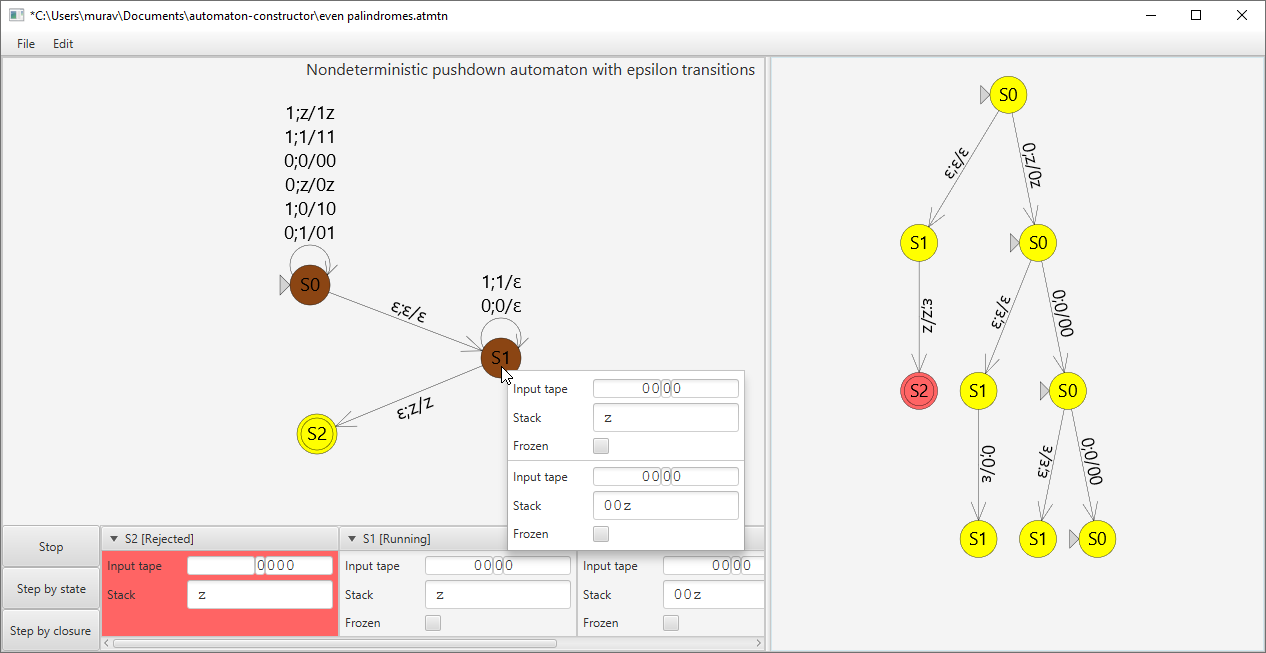
\includegraphics[width=0.9\textwidth]{debug1.png}}
        \end{frame}
        
        \begin{frame}{Обзор}
            Подробнее
            \begin{itemize}
                \item README
                    \begin{itemize}
                        \item \url{github.com/spbu-se/KotlinAutomataConstructor}
                    \end{itemize}
                \item Пользовательская документация
                    \begin{itemize}
                        \item \url{docs.google.com/document/d/1jhqQSpF-SMvZJMpAzzRWi49u15uQ_wBPstUS369gO-Y}
                    \end{itemize}
                \item Отчёты по учебной практике
                    \begin{itemize}
                        \item \url{drive.google.com/file/d/1RzXoGHFHjjEvBZPwH-dYr5N4t7hHrZaJ}
                        \item \url{drive.google.com/file/d/1sPX4CGHwINEX7otoTbet_GFub7ILjjjm}
                    \end{itemize}
            \end{itemize}
        \end{frame}
        
        \begin{frame}{Задачи на ЛШ}
            \begin{itemize}
                \item Создание вычислителей по их описанию на формальном языке
                \begin{itemize}
                    \item Для конечных автоматов --- по регулярным выражениям
                    \item Для автоматов с магазинной памятью --- по контекстно свободным грамматикам
                \end{itemize}
                \item Преобразование вычислителей одного вида в другой
                \begin{itemize}
                    \item НКА $\longrightarrow$ ДКА
                    \item Машина Мили $\longleftrightarrow$ Машина Мура
                \end{itemize}
                \item Прочая функциональность
                    \begin{itemize}
                        \item Меню <<Help>>
                        \item Ctrl+C, Ctrl+V
                        \item Локализация
                        \item Стандартная библиотека вычислителей
                    \end{itemize}
            \end{itemize}
        \end{frame}
        
        \begin{frame}{Требования к кандидату (ищем 1-3 человек)}
            Необходим
            \begin{itemize}
                \item Опыт разработки на Kotlin или желание и возможность изучить этот язык
            \end{itemize}
            \vspace{10pt}
            Плюсом будет
            \begin{itemize}
                \item Знакомство с JavaFX (TornadoFX)
                \item Умение использовать JUnit 5
            \end{itemize}
        \end{frame}
        
        \begin{frame}{Контакты для заявок}
            \begin{itemize}
                \item MS Teams: Муравьев Илья Владимирович
                \item Telegram: \href{https://t.me/ilyamuravjov}{\color{blue}{@ilyamuravjov}}
            \end{itemize}
        \end{frame}

\end{document}